\section{\protect\isl/ interface}

\let\llt\prec
\let\lle\preccurlyeq
\let\lgt\succ

\subsection{Library}

The \barvinok/ library currently supports only a few
functions that interface with the \isl/ library.
In time, this interface will grow and is set to replace
the \PolyLib/ interface.
For more information on the \isl/ data structures, see
the \isl/ user manual.

\begin{verbatim}
__isl_give isl_pw_qpolynomial *isl_basic_set_card(
        __isl_take isl_basic_set *bset);
__isl_give isl_pw_qpolynomial *isl_set_card(__isl_take isl_set *set);
__isl_give isl_union_pw_qpolynomial *isl_union_set_card(
        __isl_take isl_union_set *uset);
\end{verbatim}
Compute the number of elements in an \ai[\tt]{isl\_basic\_set},
\ai[\tt]{isl\_set} or \ai[\tt]{isl\_union\_set}.
The resulting \ai[\tt]{isl\_pw\_qpolynomial}
or \ai[\tt]{isl\_union\_pw\_qpolynomial} has purely parametric cells.

\begin{verbatim}
__isl_give isl_pw_qpolynomial *isl_basic_map_card(
        __isl_take isl_basic_map *bmap);
__isl_give isl_pw_qpolynomial *isl_map_card(__isl_take isl_map *map);
__isl_give isl_union_pw_qpolynomial *isl_union_map_card(
        __isl_take isl_union_map *umap);
\end{verbatim}
Compute a closed form expression for the number of image elements
associated to any element in the domain of the given \ai[\tt]{isl\_basic\_map},
\ai[\tt]{isl\_map} or \ai[\tt]{isl\_union\_map}.
The union of the cells in the resulting \ai[\tt]{isl\_pw\_qpolynomial}
is equal to the domain of the input \ai[\tt]{isl\_map}.

\begin{verbatim}
__isl_give isl_pw_qpolynomial *isl_pw_qpolynomial_sum(
        __isl_take isl_pw_qpolynomial *pwqp);
__isl_give isl_union_pw_qpolynomial *isl_union_pw_qpolynomial_sum(
        __isl_take isl_union_pw_qpolynomial *upwqp);
\end{verbatim}
Compute the sum of the given piecewise quasipolynomial over
all integer points in the domain.  The result is a piecewise
quasipolynomial that only involves the parameters.
If, however, the domain of the piecewise quasipolynomial wraps
a relation, then the sum is computed over all integer points
in the range of that relation and the domain of the relation
becomes the domain of the result.

\begin{verbatim}
__isl_give isl_pw_qpolynomial *isl_set_apply_pw_qpolynomial(
        __isl_take isl_set *set, __isl_take isl_pw_qpolynomial *pwqp);
__isl_give isl_union_pw_qpolynomial *isl_union_set_apply_union_pw_qpolynomial(
        __isl_take isl_union_set *uset,
        __isl_take isl_union_pw_qpolynomial *upwqp);
\end{verbatim}
Compute the sum of the given piecewise quasipolynomial over
all integer points in the intersection of the domain and the given set.

\begin{verbatim}
__isl_give isl_pw_qpolynomial *isl_map_apply_pw_qpolynomial(
        __isl_take isl_map *map, __isl_take isl_pw_qpolynomial *pwqp);
__isl_give isl_union_pw_qpolynomial *isl_union_map_apply_union_pw_qpolynomial(
        __isl_take isl_union_map *umap,
        __isl_take isl_union_pw_qpolynomial *upwqp);
\end{verbatim}
Compose the given map with the given piecewise quasipolynomial.
That is, compute the sum over all elements in the intersection
of the range of the map and the domain of the piecewise quasipolynomial
as a function of an element in the domain of the map.

\subsection{Calculator}

The \ai[\tt]{iscc} calculator offers an interface to some
of the functionality provided by the \isl/, \cloog/ and \barvinok/
libraries.
The language used by \ai[\tt]{iscc} is extremely simple.  The calculator
supports operations on constants and dynamically typed variables and
assignments (\ai[\tt]{:=}) to those variables.  If the result of an expression
is not used inside another expression and not assigned to a variable,
then this result is printed on the screen.  The operators are overloaded
based on the types of the arguments, which may be sets, relations,
piecewise quasipolynomials, piecewise quasipolynomial folds, lists,
strings or booleans.
The supported operations are shown in \autoref{t:iscc}.
Note that when an operation requires an argument of a certain
type, a binary list with the first element of the required type
may also be used instead.

\subsubsection{Sets and Iteration Domains}

\begin{figure}
\begin{lstlisting}[escapechar=@]{}
for (i = 1; i <= n; ++i)
    for (j = 1; j <= i; ++j)
        /* S */
\end{lstlisting}
\caption{A loop nest}
\label{f:loop nest}
\end{figure}

\begin{figure}
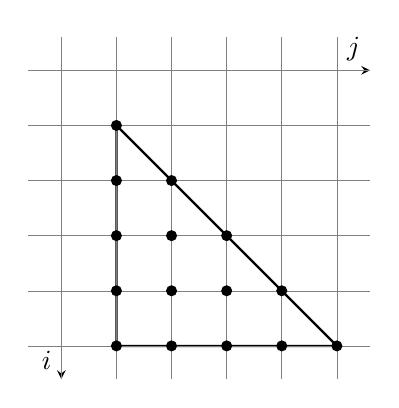
\begin{tikzpicture}[>=stealth,x=0.7cm,y=-0.7cm]
\draw[thick] (1,1)--(5,5)--(1,5)--(1,1);
\draw[->] (-0.6,0) to (5.6,0) node[anchor=south east] {$j$};
\draw[->] (0,-0.6) to (0,5.6) node[anchor=south east] {$i$};
\draw[help lines,step=0.7cm] (-0.6,5.6) grid (5.6,-0.6);
\foreach \i in {1,...,5}{
    \foreach \j in {1,...,\i}{
        \fill (\j,\i) circle (2pt);
    }
}
\end{tikzpicture}
\caption{The iteration domain of the loop nest in \autoref{f:loop nest}}
\label{f:iteration domain}
\end{figure}

Within the polyhedral model for analysis and transformation of
static affine programs, the most basic kind of set is the
\defindex{iteration domain}.
The iteration domain represents the iterations of a statement in a loop nest.
Take, for example, the loop nest in \autoref{f:loop nest}
and assume first that \lstinline{n} has a fixed value, say 5.
The pairs of values of \lstinline{i} and \lstinline{j} for
which statement \lstinline{S} is executed are shown graphically
in \autoref{f:iteration domain}.
Mathematically, this set of pairs can be represented as
$$
\{\,
(i,j) \in \ZZ^2 \mid 1 \le i \le 5 \wedge 1 \le j \le i
\,\}
$$
and the \isl/ notation is very similar:
\begin{lstlisting}[columns=flexible,escapechar=@,language=]{}
{ [i,j] : 1 <= i <= 5 and 1 <= j <= i }
\end{lstlisting}
In this notation,
the coordinates are separated by commas and enclosed in square
brackets.  This description of the space in which the set lives
is followed by a colon and the constraints on the coordinates.
Assuming the iterators are incremented by one in every iterations
of the loop, a lower and upper bound on each loop iterator
can be read off from the initialization and the test.
Note that in an \iscc/ set,
the coordinates are assumed to be integer by default.
For an iteration domain to be representable by such a set,
the iterators therefore need to be integers.

The constraints of a set need to be affine, i.e., linear plus constant term.
These affine constraint may be combined through conjunctions (\texttt{and}),
disjunctions (\texttt{or}), projections (\texttt{exists}) and
negations (\texttt{not}).
Note that the formula is immediately converted
into \indac{DNF}, so it may sometimes be more efficient
to construct a set from smaller sets by applying
basic operations such as intersection ({\tt *}),
union ({\tt +}) and difference ({\tt -}).
For example, the following square with its diagonal removed,
$$
\{\,
(i,j) \mid 0 \le i,j \le 10 \wedge \lnot (i = j)
\,\}
$$
can be constructed as
\begin{lstlisting}[columns=flexible,escapechar=@,language=]{}
{ [i,j] : 0 <= i,j <= 10 } - { [i,i] }
\end{lstlisting}
or as
\begin{lstlisting}[columns=flexible,escapechar=@,language=]{}
{ [i,j] : 0 <= i,j <= 10 and not (i = j) }
\end{lstlisting}
Note that an occurrence of a relational operator in a set description
may define several constraints, one for each pair of arguments.
The elements in a list of arguments are separated by a comma.
If there are no constraints on the coordinates, i.e., in case of
a universe set, the colon may be omitted as well.
For example
\begin{lstlisting}[columns=flexible,escapechar=@,language=]{}
{ [] }
\end{lstlisting}
represents the entire (unnamed) zero-dimensional space,
and should not be confused with
\begin{lstlisting}[columns=flexible,escapechar=@,language=]{}
{ }
\end{lstlisting}
which represents the empty set.

Returning to the iteration domain of the loop nest
in \autoref{f:loop nest}, we usually do not want to analyze
such a program for a specific value of \lstinline{n},
but instead for all possible values of \lstinline{n} at once.
A generic description of the iteration domain can be obtained
through the introduction of a (free) parameter, as in
\begin{lstlisting}[columns=flexible,escapechar=@,language=]{}
[n] -> { [i,j] : 1 <= i <= n and 1 <= j <= i }
\end{lstlisting}
The optional parameters should
be declared by placing them in a comma delimited list inside \lstinline![]!
(followed by an ``\lstinline!->!'') in front of the main set description.
The parameters are global and are identified by their names,
so the order inside the list is arbitrary.
This should be contrasted to the coordinates of a space, the names of
which are only relevant within the description of the set and which
are instead identified by their positions.
That is,
\begin{lstlisting}[columns=flexible,escapechar=@,language=]{}
[n] -> { [i,j] : 1 <= i <= n and 1 <= j <= i }
\end{lstlisting}
is equal to
\begin{lstlisting}[columns=flexible,escapechar=@,language=]{}
[n] -> { [a,b] : 1 <= a <= n and 1 <= b <= a }
\end{lstlisting}
but it is not equal to
\begin{lstlisting}[columns=flexible,escapechar=@,language=]{}
[n] -> { [j,i] : 1 <= i <= n and 1 <= j <= i }
\end{lstlisting}
(because the order of the coordinates has changed)
or
\begin{lstlisting}[columns=flexible,escapechar=@,language=]{}
[m] -> { [i,j] : 1 <= i <= m and 1 <= j <= i }
\end{lstlisting}
(because it involves a different parameter).

To plug in a particular value for a parameter, the user should
take the \ai{intersection} (\ai[\tt]{*}) with a (typically universal) set that
assigns a particular value to the parameter.
For example,
\begin{lstlisting}[columns=flexible,escapechar=@,language=]{}
S := [n] -> { [i,j] : 1 <= i <= n and 1 <= j <= i };
S * [n] -> { [i,j] : n = 5 };
\end{lstlisting}
It should be noted, though, that the result is not the same
as simply replacing \lstinline{n} by 5 as the result of the above
sequence will still have the global parameter \lstinline{n} set to 5.
To avoid this assignment, the user should instead compute
the \ai{gist} (\ai[\tt]{\%}) of the original set in the context
of setting \lstinline{n} to 5.
That is, the result of the sequence below is \lstinline{True}.
\begin{lstlisting}[columns=flexible,escapechar=@,language=]{}
S1 := { [i,j] : 1 <= i <= 5 and 1 <= j <= i };
S2 := [n] -> { [i,j] : 1 <= i <= n and 1 <= j <= i };
(S2 % [n] -> { [i,j] : n = 5}) = S1;
\end{lstlisting}

\begin{figure}
\begin{lstlisting}[escapechar=@]{}
for (i = 1; i <= n; i += 3)
    /* S */
\end{lstlisting}
\caption{A loop with non-unit stride}
\label{f:stride}
\end{figure}

If a loop has a non-unit stride as in \autoref{f:stride}
then affine constraints on the coordinates and the parameters
are not sufficient to represent the iteration domain.
What is needed is a way to express that the value of
\lstinline{i} is equal to 1 plus 3 times some integer and
this is where existentially quantified variables can be used.
Existentially quantified variables are introduced by the
\ai[\tt]{exists} keyword and followed by a colon.
They can only be used within a single disjunct.
As an example, the iteration domain of the loop in \autoref{f:stride}
can be represented as
\begin{lstlisting}[columns=flexible,escapechar=@,language=]{}
[n] -> { [i] : exists a : 1 <= i <= n and i = 1 + 3 a }
\end{lstlisting}

\begin{figure}
\begin{lstlisting}[escapechar=@]{}
for (i = 1; i <= n; ++i)
    if ((i + 1) % 5 <= 2)
	/* S */
\end{lstlisting}
\caption{A loop with a modulo condition}
\label{f:modulo}
\end{figure}

Existentially quantified variables are also useful to represent
modulo constraints.  Consider for example the loop in
\autoref{f:modulo}.  The iterator values \lstinline!i! for which
the statement \lstinline!S! is executed lie between
1 and \lstinline!n! and are such that the remainder of
\lstinline!i + 1! on division by 5 is less than or equal to 2.
The constraint $(i + 1) \bmod 5 \le 2$ can be written
as $(i + 1) - 5 \floor{\frac{i+1}5} \le 2$, where
$f = \floor{\frac{i+1}5}$ is the greatest integer part of $\frac{i+1}5$.
That is, $f$ is the unique integer value satisfying the constraints
$5 f \le i + 1$ and $5 f \ge (i+1) - 4$.
The iteration domain of the statement in \autoref{f:modulo}
can therefore be represented as
\begin{lstlisting}[columns=flexible,escapechar=@,language=]{}
[n] -> { [i] : exists f : 1 <= i <= n and (i + 1) - 5 f <= 2 and
	 (i + 1) - 4 <= 5 f <= i + 1 }
\end{lstlisting}
Since greatest integer parts occur relatively frequently, there is
a special notation for them in \isl/ using \lstinline![]!.
The above set can therefore also be represented as
\begin{lstlisting}[columns=flexible,escapechar=@,language=]{}
[n] -> { [i] : 1 <= i <= n and (i + 1) - 5 * [(i + 1)/5] <= 2 }
\end{lstlisting}
Actually, since modulos are pretty common too, \isl/ also has
a special notation for them and the set can therefore also be respresented as
\begin{lstlisting}[columns=flexible,escapechar=@,language=]{}
[n] -> { [i] : 1 <= i <= n and (i + 1) % 5 <= 2 }
\end{lstlisting}
It should be noted that \lstinline![]! always rounds down
(towards $-\infty$), while integer division in C truncates
(towards 0).  When translating conditions in C containing integer
divisions and/or modulos to \isl/ constraints, the user should therefore
make sure the sign of the dividend is positive.  If not, the integer
division needs to be translated differently for positive and negative
values.

\begin{figure}
\begin{lstlisting}[escapechar=@]{}
for (i = 0; i < n; ++i)
T:  t[i] = a[i];
for (i = 0; i < n; ++i)
    for (j = 0; j < n - i; ++j)
F:      t[j] = f(t[j], t[j+1]);
for (i = 0; i < n; ++i)
B:  b[i] = t[i];
\end{lstlisting}
\caption{A program with three loop nests}
\label{f:three loops}
\end{figure}

Most programs involve more than one statement.
Although it is possible to work with different sets, each
representing the iteration domain of a statement,
it is usually more convenient to collect all iteration domains
in a single set.  To be able to differentiate between iterations
of different statements with the same values for the iterators,
\isl/ allows spaces to be named.  The name is placed in front
of the \lstinline![]! enclosing the iterators.
Consider for example the program in \autoref{f:three loops}.
The program contains three statements which have been labeled
for convenience.
The iteration domain of the first statement (\lstinline!T!)
can be represented as
\begin{lstlisting}[columns=flexible,escapechar=@,language=]{}
[n] -> { T[i] : 0 <= i < n }
\end{lstlisting}
The union of all iteration domains can be represented as
\begin{lstlisting}[columns=flexible,escapechar=@,language=]{}
[n] -> {
    T[i] : 0 <= i < n;
    F[i,j] : 0 <= i < n and 0 <= j < n - i;
    B[i] : 0 <= i < n
}
\end{lstlisting}
The semicolon \lstinline{;} is used to express a disjunction
between spaces.  This should be contrasted with the \lstinline{or}
keyword which expresses a disjunction between conjunctions of constraints.
For example, the result of the following \iscc/ statement is
\lstinline{True}.
\begin{lstlisting}[columns=flexible,escapechar=@,language=]{}
{ [i] : i = 3 or i = 5 } = { [3]; [5] };
\end{lstlisting}

\subsubsection{Maps and Access Relations}

A second important concept in the polyhedral model is that
of an \defindex{access relation}.
An access relation connects iterations of a statement
to the array elements accessed by those iterations.
Such a binary relation can be represented by a map in \isl/.
Maps are defined in similar way to sets,
except that the single space is replaced by a pair of spaces separated
by \verb!->!.
As an example, consider once more the program in \autoref{f:three loops}.
In particular, consider the access \lstinline{t[j+1]} in
statement \lstinline{F}.
The index expression maps the pair of iterations \lstinline{i}
and \lstinline{j} to \lstinline{t[j+1]}, i.e., element \lstinline{j+1}
of a space with name \lstinline{t}.
Ignoring the loop bound constraints, this access relation can
be represented as
\begin{lstlisting}[columns=flexible,escapechar=@,language=]{}
{ F[i,j] -> t[j + 1] }
\end{lstlisting}
It is however customary to include the constraints on the iterators
in the access relation, resulting in
\begin{lstlisting}[columns=flexible,escapechar=@,language=]{}
[n] -> { F[i,j] -> t[j + 1] : 0 <= i < n and 0 <= j < n - i }
\end{lstlisting}
The constraints can be added by intersecting the domains
of the access relations with the iteration domains.
For example, the following sequence constructs the access
relation for all reads in the program.
\begin{lstlisting}[columns=flexible,escapechar=@,language=]{}
D := [n] -> {
    T[i] : 0 <= i < n;
    F[i,j] : 0 <= i < n and 0 <= j < n - i;
    B[i] : 0 <= i < n
};
Read := {
    T[i] -> a[i];
    F[i,j] -> t[j];
    F[i,j] -> t[j + 1];
    B[i] -> t[i]
};
Read := Read * D;
\end{lstlisting}
In this sequence, the \lstinline{*} operator, when applied
to a map and a set, intersects the domain of the map with the set.

The notation \lstinline{R(S)} can be used to compute the image
of the set \lstinline{S} under the map \lstinline{R}.
For example, given the sequence above, \lstinline!Read({F[0,1]})!
computes the array elements read in iteration $(0,1)$ of statement
\lstinline{F} and is equal to
\begin{lstlisting}[columns=flexible,escapechar=@,language=]{}
[n] -> { t[2] : n >= 2; t[1] : n >= 2 }
\end{lstlisting}
That is, elements 1 and 2 of the \lstinline{t} array are read,
provided \lstinline{n} is at least 2.

Maps need not be single-valued.
As an example, assume that \lstinline{A} is a two-dimensional
array of size \lstinline{n} in both dimensions.
Iterations \lstinline{i} of
a statement \lstinline{S} may pass a pointer to an entire row
of \lstinline{A} to a function as in \lstinline{f(A[i])}.
Without knowing anything about \lstinline{f}, we would have
to assume that this function may access any element of the row.
The access relation corresponding to \lstinline{A[i]} is therefore
\begin{lstlisting}[columns=flexible,escapechar=@,language=]{}
[n] -> { S[i] -> A[i,j] : 0 <= i,j < n }
\end{lstlisting}
This map associates \lstinline{n} elements of \lstinline{A}
to each iteration of \lstinline{S}.

\subsubsection{Nested Spaces}

Each space may contain a nested pair of spaces.  Such nested spaces
are extremely useful in more advanced applications.
As an example, suppose that during equivalence checking
\shortcite{Verdoolaege2009equivalence}
of two programs the iterations of \verb!S1! in one program are supposed to
produce the same results as the same iterations of \verb!SA! in the other program,
which may be described using the following map
\begin{verbatim}
[n] -> { S1[i] -> SA[i] : 0 <= i <= n }
\end{verbatim}
If the iterations of \verb!S1! depend on the same iterations
of \verb!S2!, i.e., \verb!{S1[i]->S2[i]}!, while those of \verb!SA!
depend on the next iteration of \verb!B!, i.e., \verb!{SA[i]->SB[i+1]}!,
then we can apply the cross product of these two dependence maps, i.e.,
\begin{verbatim}
{ [S1[i] -> SA[i']] -> [S2[i] -> SB[1+i']] }
\end{verbatim}
to the original map to find
out which iterations of \verb!S2! should correspond to which
iterations of \verb!SB!.

\subsubsection{Basic Operations}

Basic operations on sets and maps include intersection (\ai[\tt]{*}),
union (\ai[\tt]{+}), difference (\ai[\tt]{-}), cross product (\ai[\tt]{cross}),
sampling (\ai[\tt]{sample}), affine hull (\ai[\tt]{aff}),
lexicographic optimization (\ai[\tt]{lexmin} or \ai[\tt]{lexmax}),
subset (\ai[\tt]{<=}) and equality (\ai[\tt]{=}) tests,
code generation (\ai[\tt]{codegen})
and the cardinality (\ai[\tt]{card}).
Additional operations on maps include computing domain (\ai[\tt]{dom})
and range (\ai[\tt]{ran}), differences between image and domain (\ai[\tt]{deltas}),
join (\ai[\tt]{.}), inverse (\ai[\tt]{\^{}-1}) and transitive closure (\ai[\tt]{\^{}+}).
The latter may result in an overapproximation.

The \ai[\tt]{card} operation computes the number of elements in a set
or the number of elements in the image of a domain element of a map.
The operation is performed exactly and completely symbolically and
the result is a piecewise quasipolynomial, i.e., a subdivision of one
or more spaces, with a quasipolynomial associated to each cell in the subdivision.
As a trivial example, the result of
\begin{verbatim}
card { A[i] -> B[j] : 0 <= j <= i }
\end{verbatim}
is \verb!{ A[i] -> (1+i) : i >= 0 }!.
Operations on piecewise quasipolynomials include sum (\ai[\tt]{+})
and difference (\ai[\tt]{-}) and the computation of an upper bound over the domain.
If the domain contains a pair of nested spaces, then the upper bound is computed over
the nested range.  As another trivial example, the result of
\begin{verbatim}
ub{ [[i] -> [j]] -> j^2 : -i <= j <= i }
\end{verbatim}
is
\verb!({ [i] -> max(i^2) : i >= 0 }, True)!.
The first element in this list is the actual bound in the form
of a piecewise quasipolynomial fold,
i.e., a maximum of quasipolynomials defined over cells.
The second indicates whether the bound is tight, i.e., whether
a maximum has been computed.

\subsubsection{Advanced Operations}

While the basic {\tt card} operation simply counts the number of elements
in an affine set, it is also possible to assign a weight to each element
of the set and to compute the sum of those weights over all the points in the set.
The syntax for this weighted counting is to compute the {\tt sum} of
a piecewise quasipolynomial over its domain.  As in the case of the {\tt ub}
operator, if the domain contains a pair of nested space, the sum is computed
over the range.  As an example, the result
of
\begin{verbatim}
sum{ [[i] -> [j]] -> i*j : 0 <= j <= i }
\end{verbatim}
is
\verb|{ [i] -> (1/2*i^2+1/2*i^3) : i >= 0 }|.

After the computation of some sum or bound, the result may have to
be reformulated in terms of other variables.  For example, during
inter procedural analysis, a result computed in terms of the formal
parameters may have to be reformulated in terms of the actual parameters.
{\tt iscc} therefore allows maps and
piecewise quasipolynomials or folds to be composed.
If the map is multi-valued, then the composition maps each domain element
to the sum or upper bound of the values at its image elements.

Finally, because of its high-level representation, {\tt iscc} can
provide a dependence analysis operation taking only three maps as input,
the sink accesses, the potential source accesses and a schedule.
The result is a single dependence map.


\subsubsection{More Examples}
\begin{verbatim}
P := [n, m] -> { [i,j] : 0 <= i <= n and i <= j <= m };
card P;

f := [n,m] -> { [i,j] -> i*j + n*i*i*j : i,j >= 0 and 5i + 27j <= n+m };
sum f;
s := sum f;
s @ [n,m] -> { : 0 <= n,m <= 20 };

f := [n] -> { [i] -> 2*n*i - n*n + 3*n - 1/2*i*i - 3/2*i-1 :
                (exists j : 0 <= i < 4*n-1 and 0 <= j < n and
                            2*n-1 <= i+j <= 4*n-2 and i <= 2*n-1 ) };
ub f;
u := (ub f)[0];
u @ [n] -> { : 0 <= n <= 10 };

m := [n] -> { [i,j] -> [i+1,j+1] : 1 <= i,j < n;
              [i,j] -> [i+1,j-1] : 1 <= i < n and 2 <= j <= n };
m^+;
(m^+)[0];

codegen [N] -> { A[i] -> [i,0] : 0 <= i <= N; B[i] -> [i,1] : 1 <= i <= N };

{ [k] -> [i] : 1 <= i <= k } . { [n] -> 2 * n : n >= 1 };

{ [m] -> [c] : 1 <= c <= m } . { [k] -> max((3 * k + k^2)) : k >= 1 };
\end{verbatim}

\subsubsection{Comparison to other Interactive Polyhedral Tools}

Two related interactive polyhedral tools are
the Omega calculator \shortcite{Omega_calc}
and {\tt SPPoC} \shortcite{Boulet2001SPPoC}.
The syntax of {\tt iscc} was very much inspired
by that of the Omega calculator.  However, the Omega
calculator only knows sets and maps.  In particular,
it does not perform any form of counting.  An earlier version
of \barvinok/ came with a modified version of
the Omega calculator that introduced an operation
for counting the number of elements in a set, but it
would simply print the result and not allow any further
manipulations.
{\tt SPPoC} does support counting, but only the basic
operation of counting the elements in a set.
In particular, it does not support weighted counting,
nor the computation of upper bounds.
It also only supports (single-valued) functions
and not generic relations like the Omega calculator and {\tt iscc}.
Internally, {\tt SPPoC} uses {\tt PolyLib}, {\tt PipLib} and {\tt omega}
to perform
its operations.  Although the first two of these libraries may have been
state-of-the-art at the time {\tt SPPoC} was created, they are
no longer actively maintained and have been largely
superseded by more recent libraries.
In particular, {\tt PipLib} effectively only supports a single
operation, which is now also available in both {\tt isl} and {\tt PPL}.
The operations on rational polyhedra in {\tt PolyLib} are also
available in {\tt PPL}, usually through a cleaner interface and
with a more efficient implementation.  As to counting the elements
in a parametric polytope, Barvinok's algorithm,
implemented in the {\tt barvinok} library, is usually much faster
than the algorithm implemented in {\tt PolyLib}
\shortcite{Verdoolaege2007parametric}.
Furthermore,
the ability to work with named and nested spaces and the ability
of sets and maps to contain (pairs of) elements from different spaces
are not available in the Omega calculator and {\tt SPPoC}.

\newpage
\tablecaption{{\tt iscc} operations.  The variables
have the following types,
$s$: set,
$m$: map,
$q$: piecewise quasipolynomial,
$f$: piecewise quasipolynomial fold,
$l$: list,
$i$: integer,
$b$: boolean,
$S$: string,
$o$: object of any type
}
\label{t:iscc}
\tablehead{
\hline
Syntax & Meaning
\\
\hline
}
\tabletail{
\multicolumn{2}{r}{\small\sl continued on next page}
\\
}
\tablelasttail{}
\begin{supertabular}{p{0.35\textwidth}p{0.6\textwidth}}
$s_2$ := \ai[\tt]{aff} $s_1$ & affine hull of $s_1$
\\
$m_2$ := \ai[\tt]{aff} $m_1$ & affine hull of $m_1$
\\
$q$ := \ai[\tt]{card} $s$ &
number of elements in the set $s$
\\
$q$ := \ai[\tt]{card} $m$ &
number of elements in the image of a domain element
\\
$s_2$ := \ai[\tt]{coalesce} $s_1$ &
simplify the representation of set $s_1$ by trying
to combine pairs of basic sets into a single
basic set
\\
$m_2$ := \ai[\tt]{coalesce} $m_1$ &
simplify the representation of map $m_1$ by trying
to combine pairs of basic maps into a single
basic map
\\
$q_2$ := \ai[\tt]{coalesce} $q_1$ &
simplify the representation of $q_1$ by trying
to combine pairs of basic sets in the domain
of $q_1$ into a single basic set
\\
$f_2$ := \ai[\tt]{coalesce} $f_1$ &
simplify the representation of $f_1$ by trying
to combine pairs of basic sets in the domain
of $f_1$ into a single basic set
\\
\ai[\tt]{codegen} $s$ &
generate code for the given domain.
This operation is only available if \ai[\tt]{CLooG}
support was compiled in.
\\
\ai[\tt]{codegen} $m$ &
generate code for the given scattering function.
This operation is only available if \ai[\tt]{CLooG}
support was compiled in.
\\
$s_2$ := \ai[\tt]{coefficients} $s_1$ &
The set of coefficients of valid constraints for $s_1$
\\
$s_2$ := \ai[\tt]{solutions} $s_1$ &
The set of elements satisfying the constraints with coefficients in $s_1$
\\
$s_3$ := $s_1$ \ai[\tt]{cross} $s_2$ &
Cartesian product of $s_1$ and $s_2$
\\
$m_3$ := $m_1$ \ai[\tt]{cross} $m_2$ &
Cartesian product of $m_1$ and $m_2$
\\
$s$ := \ai[\tt]{deltas} $m$ &
the set $\{\, y - x \mid x \to y \in m \,\}$
\\
$m_2$ := \ai[\tt]{deltas\_map} $m_1$ &
the map $\{\, (x \to y) \to y - x \mid x \to y \in m_1 \,\}$
\\
$s$ := \ai[\tt]{dom} $m$ &
domain of map $m$
\\
$s$ := \ai[\tt]{dom} $q$ &
domain of piecewise quasipolynomial $q$
\\
$s$ := \ai[\tt]{dom} $f$ &
domain of piecewise quasipolynomial fold $f$
\\
$s$ := \ai[\tt]{domain} $m$ &
domain of map $m$
\\
$s$ := \ai[\tt]{domain} $q$ &
domain of piecewise quasipolynomial $q$
\\
$s$ := \ai[\tt]{domain} $f$ &
domain of piecewise quasipolynomial fold $f$
\\
$m_2$ := \ai[\tt]{domain\_map} $m_1$ &
a map from a wrapped copy of $m_1$ to the domain of $m_1$
\\
$s$ := \ai[\tt]{ran} $m$ &
range of map $m$
\\
$s$ := \ai[\tt]{range} $m$ &
range of map $m$
\\
$m_2$ := \ai[\tt]{range\_map} $m_1$ &
a map from a wrapped copy of $m_1$ to the range of $m_1$
\\
$m$ := \ai[\tt]{identity} $s$ &
identity relation on $s$
\\
$q$ := \ai[\tt]{lattice\_width} $s$ &
lattice width of the set $s$
\\
$s_2$ := \ai[\tt]{lexmin} $s_1$ &
lexicographically minimal element of $s_1$
\\
$m_2$ := \ai[\tt]{lexmin} $m_1$ &
lexicographically minimal image element
\\
$s_2$ := \ai[\tt]{lexmax} $s_1$ &
lexicographically maximal element of $s_1$
\\
$m_2$ := \ai[\tt]{lexmax} $m_1$ &
lexicographically maximal image element
\\
$s_2$ := \ai[\tt]{lift} $s_1$ &
lift $s_1$ to a space with extra dimensions corresponding
to the existentially quantified variables in $s_1$ such
that \lstinline!domain(unwrap(lift S))! is equal to \lstinline!S!
\\
$l$ := \ai[\tt]{parse\_file} $S$ &
parse the file names $S$ and return a list consisting of
the iteration domains, the write access relations,
the read access relations and the original schedule.
This operation is only available if \ai[\tt]{pet}
support was compiled in.
\\
$s_2$ := \ai[\tt]{poly} $s_1$ & polyhedral hull of $s_1$
\\
$m_2$ := \ai[\tt]{poly} $m_1$ & polyhedral hull of $m_1$
\\
$q_2$ := \ai[\tt]{poly} $q_1$ & polynomial approximation of $q_1$
\\
$q_2$ := \ai[\tt]{lpoly} $q_1$ & polynomial underapproximation of $q_1$
\\
$q_2$ := \ai[\tt]{upoly} $q_1$ & polynomial overapproximation of $q_1$
\\
$l$ := \ai[\tt]{pow} $m$\ &
compute an overapproximation of the power
of $m$ and return a list containing the overapproximation
and a boolean that is true if the overapproximation
is known to be exact
\\
\ai[\tt]{print} $o$ &
print object
\\
$o$ := \ai[\tt]{read} {\tt "}{\it filename}{\tt"} &
read object from file
\\
$s_2$ := \ai[\tt]{sample} $s_1$ &
a sample element of the set $s_1$
\\
$m_2$ := \ai[\tt]{sample} $m_1$ &
a sample element of the map $m_1$
\\
$s_2$ := \ai[\tt]{scan} $s_1$ &
the set $s_1$ split into individual elements,
provided $s_1$ contains a finite number of elements
\\
$m_2$ := \ai[\tt]{scan} $m_1$ &
the map $m_1$ split into individual elements,
provided $m_1$ contains a finite number of elements
\\
\ai[\tt]{source} {\tt "}{\it filename}{\tt"} &
read commands from file
\\
$q_2$ := \ai[\tt]{sum} $q_1$ &
sum $q_1$ over all integer points in the domain of $q_1$,
or, if the domain of $q_1$ wraps a map, over all integer
points in the range of the wrapped map.
\\
$S$ := \ai[\tt]{typeof} $o$ &
a string representation of the type of $o$
\\
$l$ := \ai[\tt]{ub} $q$ &
compute an
upper bound on the piecewise quasipolynomial $q$ over
all integer points in the domain of $q$
and return a list containing the upper bound
and a boolean that is true if the upper bound
is known to be tight.
If the domain of $q$ wraps a map, then the upper
bound is computed over all integer points in
the range of the wrapped map instead.
\\
$l$ := \ai[\tt]{vertices} $s$ &
a list of vertices of the rational polytope defined by the same constraints
as $s$
\\
$s$ := \ai[\tt]{wrap} $m$ &
wrap the map in a set
\\
$m$ := \ai[\tt]{unwrap} $s$ &
unwrap the map from the set
\\
\ai[\tt]{write} {\tt "}{\it filename}{\tt"} $o$ &
write object to file
\\
$m_2$ := \ai[\tt]{zip} $m_1$ &
the cross product of domain and range of $m_1$, i.e.,
$\{\, (\vec w \to \vec y) \to (\vec x \to \vec z)
\mid (\vec w \to \vec x) \to (\vec y \to \vec z) \in m_1 \,\}$
\\
$m_4$ := \ai[\tt]{any} $m_1$ \ai[\tt]{before} $m_2$ \ai[\tt]{under} $m_3$ &
compute a map from any element $x$ in the domain of $m_1$
to any element $y$ in the domain of $m_2$
such that their images $m_1(x)$ and $m_2(y)$ overlap
and such that $m_3(x) \llt m_3(y)$.
\\
$l$ := \ai[\tt]{last} $m_1$ \ai[\tt]{before} $m_2$ \ai[\tt]{under} $m_3$ &
compute a map that contains for any element $y$ in the domain of $m_2$
a mapping from the lexicographically last element $x$ in the domain of $m_1$
(according to the schedule $m_3$) to $y$
such that $m_1(x)$ and $m_2(y)$ overlap and such that $m_3(x) \llt m_3(y)$.
Return a list containing this map and the set of elements in the domain of
$m_2$ for which there is no corresponding element in the domain of $m_1$.
\\
$m_5$ := \ai[\tt]{any} $m_1$ \ai[\tt]{last} $m_2$ \ai[\tt]{before} $m_3$
\ai[\tt]{under} $m_4$ &
compute a map that contains for any element $y$ in the domain of $m_3$
a mapping from the lexicographically last element $x$ in the domain of $m_2$
(according to the schedule $m_4$) to $y$
such that $m_2(x)$ and $m_3(y)$ overlap and such that $m_4(x) \llt m_4(y)$
as well as from any element $z$ in the domain of $m_1$ such that
$m_1(z)$ and $m_3(y)$ overlap, $m_4(z) \llt m_4(y)$ and such that there
is no $x$ in the domain of $m_2$ with
$m_2(x) \cap m_3(y) \ne \emptyset$ and $m_4(z) \llt m_4(x) \llt m_4(y)$.
\\
$m_3$ := \ai[\tt]{schedule} $s$ \ai[\tt]{respecting} $m_1$ \ai[\tt]{minimizing} $m_2$ &
compute a schedule for the domains in $s$ that respects all dependences
in $m_1$ and tries to minimize the dependences in $m_2$.
\\
$l$ := \ai[\tt]{schedule\_forest} $s$ \ai[\tt]{respecting} $m_1$ \ai[\tt]{minimizing} $m_2$ &
compute a schedule for the domains in $s$ that respects all dependences
in $m_1$ and tries to minimize the dependences in $m_2$ and return
the forest of bands in the schedule.
\\
$i_3$ := $i_1$ \ai{$+$} $i_2$ & sum
\\
$s_3$ := $s_1$ \ai{$+$} $s_2$ & union
\\
$m_3$ := $m_1$ \ai{$+$} $m_2$ & union
\\
$q_3$ := $q_1$ \ai{$+$} $q_2$ & sum
\\
$f_2$ := $f_1$ \ai{$+$} $q$ & sum
\\
$f_2$ := $q$ \ai{$+$} $f_1$ & sum
\\
$S_3$ := $S_1$ \ai{$+$} $S_2$ & concatenation
\\
$S_2$ := $o$ \ai{$+$} $S_1$ &
concatenation of stringification of $o$ and $S_1$
\\
$S_2$ := $S_1$ \ai{$+$} $o$ &
concatenation of $S_1$ and stringification of $o$
\\
$i_3$ := $i_1$ \ai{$-$} $i_2$ & difference
\\
$s_3$ := $s_1$ \ai{$-$} $s_2$ & set difference
\\
$m_3$ := $m_1$ \ai{$-$} $m_2$ & set difference
\\
$q_3$ := $q_1$ \ai{$-$} $q_2$ & difference
\\
$i_3$ := $i_1$ \ai{$*$} $i_2$ & product
\\
$s_3$ := $s_1$ \ai{$*$} $s_2$ & intersection
\\
$m_3$ := $m_1$ \ai{$*$} $m_2$ & intersection
\\
$q_2$ := $i$ \ai{$*$} $q_1$ & product
\\
$q_2$ := $q_1$ \ai{$*$} $i$ & product
\\
$q_3$ := $q_1$ \ai{$*$} $q_2$ & product
\\
$f_2$ := $i$ \ai{$*$} $f_1$ & product
\\
$f_2$ := $f_1$ \ai{$*$} $i$ & product
\\
$m_2$ := $m_1$ \ai{$*$} $s$ & intersect domain of $m_1$ with $s$
\\
$q_2$ := $q_1$ \ai{$*$} $s$ & intersect domain of $q_1$ with $s$
\\
$f_2$ := $f_1$ \ai{$*$} $s$ & intersect domain of $f_1$ with $s$
\\
$s_2$ := $m$($s_1$) & apply map $m$ to set $s_1$
\\
$q_2$ := $q_1$($s$) & apply $q_1$ to each element in $s$ and compute
the sum of the results
\\
$l$ := $f$($s$) & apply $f$ to each element in $s$, compute
a bound of the results
and return a list containing the bound
and a boolean that is true if the bound
is known to be tight.
\\
$m_3$ := $m_1$ \ai[\tt]{.} $m_2$ & join of $m_1$ and $m_2$
\\
$m_3$ := $m_1$ \ai[\tt]{before} $m_2$ & join of $m_1$ and $m_2$
\\
$m_3$ := $m_2$($m_1)$ & join of $m_1$ and $m_2$
\\
$m_3$ := $m_2$ \ai[\tt]{after} $m_1$ & join of $m_1$ and $m_2$
\\
$f_3$ := $f_1$ \ai[\tt]{.} $f_2$ & join of $f_1$ and $f_2$, combining
the lists of quasipolynomials over shared domains
\\
$q_2$ := $m$ \ai[\tt]{.} $q_1$ & join of $m$ and $q_1$, taking the sum
over all elements in the intersection of the range of $m$ and the domain
of $q_1$
\\
$q_2$ := $m$ \ai[\tt]{before} $q_1$ & $q_2$ := $m$ \ai[\tt]{.} $q_1$
\\
$q_2$ := $q_1(m)$ & $q_2$ := $m$ \ai[\tt]{.} $q_1$
\\
$q_2$ := $q_1$ \ai[\tt]{after} $m$ & $q_2$ := $m$ \ai[\tt]{.} $q_1$
\\
$l$ := $m$ \ai[\tt]{.} $f$ & join of $m$ and $f$, computing a bound
over all elements in the intersection of the range of $m$ and the domain
of $f$ and returning a list containing the bound
and a boolean that is true if the bound is known to be tight.
\\
$l$ := $m$ \ai[\tt]{before} $f$ & $l$ := $m$ \ai[\tt]{.} $f$
\\
$l$ := $f(m)$ & $l$ := $m$ \ai[\tt]{.} $f$
\\
$l$ := $f$ \ai[\tt]{after} $m$ & $l$ := $m$ \ai[\tt]{.} $f$
\\
$m$ := $s_1$ \ai[\tt]{->} $s_2$ & universal map with domain $s_1$
and range $s_2$
\\
$q_2$ := $q_1$ \ai{@} $s$ &
evaluate the piecewise quasipolynomial $q_1$ in each element
of the set $s$ and return a piecewise quasipolynomial
mapping each of the individual elements to the resulting
constant
\\
$q$ := $f$ \ai{@} $s$ &
evaluate the piecewise quasipolynomial fold $f$ in each element
of the set $s$ and return a piecewise quasipolynomial
mapping each of the individual elements to the resulting
constant
\\
$s_3$ := $s_1$ \ai[\tt]{\%} $s_2$ &
simplify $s_1$ in the context of $s_2$, i.e., compute
the gist of $s_1$ given $s_2$
\\
$m_3$ := $m_1$ \ai[\tt]{\%} $m_2$ &
simplify $m_1$ in the context of $m_2$, i.e., compute
the gist of $m_1$ given $m_2$
\\
$m_2$ := $m_1$ \ai[\tt]{\%} $s$ &
simplify $m_1$ in the context of the domain $s$, i.e., compute
the gist of $m_1$ given domain $s$
\\
$q_2$ := $q_1$ \ai[\tt]{\%} $s$ &
simplify $q_1$ in the context of the domain $s$, i.e., compute
the gist of $q_1$ given $s$
\\
$f_2$ := $f_1$ \ai[\tt]{\%} $s$ &
simplify $f_1$ in the context of the domain $s$, i.e., compute
the gist of $f_1$ given $s$
\\
$m_2$ := $m_1$\ai[\tt]{\^{}-1} & inverse of $m_1$
\\
$l$ := $m$\ai[\tt]{\^{}+} &
compute an overapproximation of the transitive closure
of $m$ and return a list containing the overapproximation
and a boolean that is true if the overapproximation
is known to be exact
\\
$o$ := $l$[$i$] &
the element at position $i$ in the list $l$
\\
$b$ := $q_1$ \ai[\tt]{==} $q_2$ & is $q_1$ obviously equal to $q_2$?
\\
$b$ := $f_1$ \ai[\tt]{==} $f_2$ & is $f_1$ obviously equal to $f_2$?
\\
$b$ := $s_1$ \ai[\tt]{=} $s_2$ & is $s_1$ equal to $s_2$?
\\
$b$ := $m_1$ \ai[\tt]{=} $m_2$ & is $m_1$ equal to $m_2$?
\\
$b$ := $s_1$ \ai[\tt]{<=} $s_2$ & is $s_1$ a subset of $s_2$?
\\
$b$ := $m_1$ \ai[\tt]{<=} $m_2$ & is $m_1$ a subset of $m_2$?
\\
$b$ := $s_1$ \ai[\tt]{<} $s_2$ & is $s_1$ a proper subset of $s_2$?
\\
$b$ := $m_1$ \ai[\tt]{<} $m_2$ & is $m_1$ a proper subset of $m_2$?
\\
$b$ := $s_1$ \ai[\tt]{>=} $s_2$ & is $s_1$ a superset of $s_2$?
\\
$b$ := $m_1$ \ai[\tt]{>=} $m_2$ & is $m_1$ a superset of $m_2$?
\\
$b$ := $s_1$ \ai[\tt]{>} $s_2$ & is $s_1$ a proper superset of $s_2$?
\\
$b$ := $m_1$ \ai[\tt]{>} $m_2$ & is $m_1$ a proper superset of $m_2$?
\\
$m$ := $s_1$ \ai[\tt]{<<} $s_2$ & a map from
$s_1$ to $s_2$ of those elements that live in the same space and
such that the elements of $s_1$ are lexicographically strictly smaller
than those of $s_2$.
\\
$m_3$ := $m_1$ \ai[\tt]{<<} $m_2$ & a map from the domain of
$m_1$ to the domain of $m_2$ of those elements such that their images
live in the same space and such that the images of the elements of
$m_1$ are lexicographically strictly smaller than those of $m_2$.
\\
$m$ := $s_1$ \ai[\tt]{<<=} $s_2$ & a map from
$s_1$ to $s_2$ of those elements that live in the same space and
such that the elements of $s_1$ are lexicographically smaller
than those of $s_2$.
\\
$m_3$ := $m_1$ \ai[\tt]{<<=} $m_2$ & a map from the domain of
$m_1$ to the domain of $m_2$ of those elements such that their images
live in the same space and such that the images of the elements of
$m_1$ are lexicographically smaller than those of $m_2$.
\\
$m$ := $s_1$ \ai[\tt]{>>} $s_2$ & a map from
$s_1$ to $s_2$ of those elements that live in the same space and
such that the elements of $s_1$ are lexicographically strictly greater
than those of $s_2$.
\\
$m_3$ := $m_1$ \ai[\tt]{>>} $m_2$ & a map from the domain of
$m_1$ to the domain of $m_2$ of those elements such that their images
live in the same space and such that the images of the elements of
$m_1$ are lexicographically strictly greater than those of $m_2$.
\\
$m$ := $s_1$ \ai[\tt]{>>=} $s_2$ & a map from
$s_1$ to $s_2$ of those elements that live in the same space and
such that the elements of $s_1$ are lexicographically greater
than those of $s_2$.
\\
$m_3$ := $m_1$ \ai[\tt]{>>=} $m_2$ & a map from the domain of
$m_1$ to the domain of $m_2$ of those elements such that their images
live in the same space and such that the images of the elements of
$m_1$ are lexicographically greater than those of $m_2$.
\\
\end{supertabular}
